
%%%%%%%%%%%%%%%%%%%%%%%%%%%%%%%%%%%%%%%%%%%%%%%%%%%%%%%%%%
%%
%%  PROJECT: Noncommutative Geometry & Diffeology: The Case Of Orbifolds
%%  FILENAME: NCGADTCOO.tex
%%
%%  Original Authors: Patrick Iglesias-Zemmour & Jean-Pierre Laffineur
%%  Modernized for the Diffeology Archives in December 2025.
%%
%%  This is a self-contained document. All necessary macros
%%  and packages are included in this preamble.
%%
%%%%%%%%%%%%%%%%%%%%%%%%%%%%%%%%%%%%%%%%%%%%%%%%%%%%%%%%%%

\documentclass[11pt,reqno]{amsart}

%%====================================================================
% MARK: - Preamble (Self-Contained)
%%====================================================================

% --- Core Packages ---
\usepackage{amsmath}
\usepackage{amssymb}
\usepackage{amscd}
\usepackage[hidelinks]{hyperref}

% --- Typography and Layout ---
\usepackage[T1]{fontenc}
\usepackage[utf8]{inputenc}
\usepackage{microtype}
% Note: uppercase=upright handles the roman math capitals automatically
\usepackage[cal=scr,sfscaled=true,frenchmath,uppercase=upright,greeklowercase=upright,greekfamily=didot,utopia]{mathdesign}
\usepackage[lining]{ebgaramond}
\linespread{1.1}
\parindent 0mm
\parskip .5ex plus 2pt

% --- Figures and Diagrams ---
\usepackage{tikz-cd}
\usetikzlibrary{calc}

% --- Theorem Environments (Specific to this paper) ---
\newtheoremstyle{article}{7pt}{7pt}{}{0pt}{\bf}{.\ }{0pt}{}
\theoremstyle{article}
\newtheorem{article}{}
\renewenvironment{proof}{\noindent \textit{Proof.}}{\nolinebreak\hfill $\square$}

% --- Minimal Set of Required Macros ---

% Standard Number Sets
\newcommand{\CC}{\mathbf C}
\newcommand{\GG}{\mathbf{G}}
\newcommand{\QQ}{\mathbf{Q}}
\newcommand{\RR}{\mathbf{R}}
\newcommand{\xZZ}{\mathbf{Z}}

% Calligraphic Letters
\newcommand{\cA}{{\mathcal A}} \newcommand{\cB}{{\mathcal B}} \newcommand{\cC}{{\mathcal C}}
\newcommand{\cF}{{\mathcal F}} \newcommand{\cN}{{\mathcal N}} \newcommand{\cO}{{\mathcal O}}
\newcommand{\cQ}{{\mathcal Q}} \newcommand{\cU}{{\mathcal U}} \newcommand{\cV}{{\mathcal V}}

% Fraktur Letters
\newcommand{\fA}{{\mathfrak A}}
\newcommand{\fF}{{\mathfrak F}}
\newcommand{\fG}{{\mathfrak G}}

% Mathematical Operators
\DeclareMathOperator{\class}{class}
\DeclareMathOperator{\Cinfty}{\mathrm{C}^\infty}
\DeclareMathOperator{\codom}{codom}
\DeclareMathOperator{\Diff}{Diff}
\DeclareMathOperator{\D}{D}
\DeclareMathOperator{\dom}{dom}
\DeclareMathOperator{\ev}{ev}
\DeclareMathOperator{\germ}{germ}
\DeclareMathOperator{\GL}{GL}
\DeclareMathOperator{\Mor}{Mor}
\DeclareMathOperator{\Obj}{Obj}
\DeclareMathOperator{\pr}{pr}
\DeclareMathOperator{\SO}{SO}
\DeclareMathOperator{\src}{src}
\DeclareMathOperator{\Stab}{Stab}
\DeclareMathOperator{\tr}{tr}
\DeclareMathOperator{\trg}{trg}

% Helper Macros
\def\artlabel[#1]{{\sc #1}}
\newcommand{\art}[1]{(art. \ref{#1})}
\newcommand{\id}{\mathbf 1}
\newcommand{\loc}{\mathrm{loc}}
\renewcommand{\emptyset}{\varnothing}
\renewcommand{\gg}{\mathbf{g}}

%%%%%%%%%%%%%%%%%%%%%%%%%%%%%%%%%%%%%%%%%%%%%%%%%%%%%%%%%%
%%
%% MARK: Document Information
%%
%%%%%%%%%%%%%%%%%%%%%%%%%%%%%%%%%%%%%%%%%%%%%%%%%%%%%%%%%%

\begin{document}

\title[Noncommutative Geometry \& Diffeology\,: The Case Of Orbifolds]{Noncommutative Geometry \& Diffeology\,: \\ The Case Of Orbifolds}

\author{Patrick Iglesias-Zemmour}
\author{Jean-Pierre Laffineur}
\date{23 March, 2017}

\address{P.I-Z --- Institut de Mathématique de Marseille,
CNRS,
France \
\& \ The Hebrew University of Jerusalem,
Israel.}
\email{piz@math.huji.ac.il}

\address{J-P.L --- Paris-Diderot University,
France.}
\email{laffineur@math.univ-paris-diderot.fr}

\keywords{Noncommutative Geometry, Diffeology, Orbifolds}

\subjclass[2010]{Primary 53C; Secondary 58B34, 57R18}

\maketitle

%%%%%%%%%%%%%%%%%%%%%%%%%%%%%%%%%%%%%%%%%%%%%%%%%%%%%%%%%%
%%
%% MARK: Abstract
%%
%%%%%%%%%%%%%%%%%%%%%%%%%%%%%%%%%%%%%%%%%%%%%%%%%%%%%%%%%%

\begin{abstract}
  We establish a first structural link between noncommutative geometry and diffeology,
  in the particular case of orbifolds.
  Precisely,
  we associate a \emph{structure groupoid} with every atlas of a diffeological orbifold.
  We show that different atlases give equivalent groupoids,
  that generates strongly Morita equivalent $\CC^*$-algebras,
  according to standards.
  Thus,
  diffeomorphisms translate naturally into Morita equivalences.
\end{abstract}

%%%%%%%%%%%%%%%%%%%%%%%%%%%%%%%%%%%%%%%%%%%%%%%%%%%%%%%%%%
%%
%% MARK: Introduction
%%
%%%%%%%%%%%%%%%%%%%%%%%%%%%%%%%%%%%%%%%%%%%%%%%%%%%%%%%%%%
\section*{Introduction}

This paper describes a first structural bridge between noncommutative geometry and diffeology%
\footnote{Non commutative geometry has been invented by Alain Connes \cite{AC80} and diffeology has been founded by Jean-Marie Souriau \cite{Sou80}.}.
The question of a relationship between these two theories appeared already at their beginnings,
in the eighties,
with the case of the \emph{irrational torus} in 1983 \cite{PDPI83, PDPI85}.
Surprisingly the analysis of the \emph{singular quotient} $T_\alpha=T^2/\Delta_\alpha$,
where $\Delta_\alpha$ is the line of irrational slope $\alpha$,
shows a highly non trivial diffeology.
In particular,
two irrational tori $T_\alpha$ and $T_\beta$ would be diffeomorphic (isomorphic in the Category \{Diffeology\}) if and only if the two numbers $\alpha$ and $\beta$ would be conjugate modulo $\GL(2,\xZZ)$.
That was also the condition,
in noncommutative geometry,
for the $\CC^*$-algebras associated with the two foliations defined by $\Delta_\alpha$ and $\Delta_\beta$ to be Morita-equivalent \cite{MR81}.
That suggested a structural relationship between noncommutative Geometry and diffeology that was not \emph{a priori\/} obvious,
and which deserved to be explored.
But this question had been left behind since then.

Noncommutative geometry has been operating for a long time now \cite{AC95},
and diffeology has since become a mature theory \cite{PIZ13}.
It is time to do a serious comparative study.
As a first step,
we begin here considering the case of orbifolds,
as they form a nice subcategory of \{Diffeology\} \cite{IKZ10}.
Orbifolds are interesting because they are simple enough diffeological spaces without being trivial.
Their simple kind of singularities make the bridge with noncommutative geometry easy to build.
Eventually,
this case is a good introduction for the more general situations to come%
\footnote{There is a larger class of diffeological spaces for which this construction will apply,
it will be explored in the next future.}.

The association of a $\CC^*$-algebras with every diffeological orbifold,
passes through the construction of a (family of) groupoid(s)
---~one for each atlas of the orbifold~---
that retains the smooth (singular) structure of the orbifold \art{The-Structure-Groupoid-Of-An-Orbifold}.
Their detailed description is given in \art{General-Description-Of-The-Structure-Groupoid}.
These groupoids giving each of them a $\CC^*$-algebra,
by a now standard procedure,
proposed by Jean Renault: \emph{A groupoid approach to C*-Algebras} \cite{JR80}.
We show then,
as a prerequisite,
that different atlases defined equivalent groupoids in the sense of equivalence of categories,
this is the proposition \art{Equivalence-Of-Structure-Groupoids}.
But,
more importantly for our concern,
different atlases give equivalent groupoids in the sense of Muhly-Renault-Williams \cite[\textsection 2]{MRW87},
this is the proposition \art{MRW-Equivalence-Of-Structure-Groupoids}.
From the MRW-equi\-va\-len\-ce, % MRW-equivalence
we deduce that the various $\CC^*$-algebras associated with different atlases are Mori\-ta equivalent \art{The-C*-Algebra-Of-an-Orbifold}. % Morita
This is the main result of this work.
It implies in particular that diffeomorphic orbifolds have Morita equivalent associated $\CC^*$-algebras,
which was an implicit requirement,
and makes this construction completely satisfactory from a purely noncommutative geometry point of view.

However,
we postponed for a future work the question of functoriality regarding the smooth maps between orbifolds.
That is because the subtle situation concerning the status of these smooth maps in diffeology,
wich is recalled and exemplified in the Introduction.
Essentially,
not all smooth maps between orbifolds have local equivariant liftings in diffeology \cite[Example 25]{IKZ10}.
This is quite singular and absent from the usual approaches which consider only maps that have local equivariant liftings.
A complete and satisfactory implementation of functoriality should not disregard these cases.

\begin{center}
  \begin{tikzcd}
    \{\text{Diffeology}\} \supset \{\text{Orbifolds}\}
    \arrow[dr, red, start anchor={south east}, end anchor={north west}]
    & & \text{$\CC^*$-Algebras} \\
    & \text{Groupoids} \arrow[ur, red, start anchor={north east}, end anchor={south west}]
    &
  \end{tikzcd}
\end{center}

It is worth mentioning that,
contrarily to the groupoid-first approach to orbifolds,
\emph{à la} Moerdijk \cite{IM02},
we begin in this work with the smooth structure:
an orbifold is first of all a diffeological space.
Then we build the associated groupoids,
which appear as a by-products of the diffeology,
and afterward the $\CC^*$-algebra.
It is a kind of converse process,
comparable with Haefliger's construction \cite{AH84}.
In this general context,
we should mention also the work of Yael Karshon and Masrour Zoghi \cite{YKMZ12},
where they build a diffeological orbifolds from an orbifold-Lie-groupoid.

\textsc{Nota Bene} --- How to read this paper?
Except for the Introduction,
the paper is built as a succession of paragraphs simply numbered.
Each paragraph has a title that summarizes its content,
and the paragraphs are grouped together in sections defined by their titles,
which is displayed centered and followed by a header.
Some paragraphs contain just definitions or constructions,
nothing that deserves to be proved.
They are left autonomous.
Some other paragraphs contain propositions or notes that need to be proved,
they are then immediately followed by a paragraph of proofs.

\textsc{Thanks} --- Thanks to the referee who,
by his remarks,
makes our text improved with more clarity in one place and fixed a mistake somewhere else.
Thanks also to Anatole Khelif for his hint in the proof of the Lemma at\ \textsection\ref{General-Description-Of-The-Structure-Groupoid},
and to Pierre Julg and Jean Renault for their input on MRW-equivalence.

%%%%%%%%%%%%%%%%%%%%%%%%%%%%%%%%%%%%%%%%%%%%%%%%%%%%%%%%%%
%%
%% MARK: Diffeological Orbifolds
%%
%%%%%%%%%%%%%%%%%%%%%%%%%%%%%%%%%%%%%%%%%%%%%%%%%%%%%%%%%%
\section*{Diffeological Orbifolds}

We recall in this section the minimum material on orbifolds we use in this study.
Let us begin by the word \emph{orbifold},
it has been coined by William Thurston \cite{WT78} in 1978 as a replacement for \emph{V-manifold},
a concept invented by Ishiro Satake in 1956 \cite{IS56}.
Orbifolds were introduced to describe spaces that look like manifolds,
except on a few subsets,
where they look like quotients of Euclidean domains by a finite group of linear transformations.

However,
Satake was unable to give a satisfactory notion of smooth maps between orbifolds.
Indeed,
in \cite[page 469]{IS57},
he writes this footnote:
\begin{quote}
  ``\emph{The notion of $C^\infty$-map thus defined is inconvenient in the point that a composite of two $C^\infty$-maps defined in a different choice of defining families is not always a $C^\infty$ map.}''
\end{quote}

Today,
diffeology resolves perfectly this issue,
in a differential-geometry traditional way.
In the paper ``Orbifolds as Diffeologies'' \cite{IKZ10},
an $n$-orbifold is defined as a diffeological space locally diffeomorphic,
at each point,
to some quotient $\RR^n/\Gamma$,
where $\Gamma \subset \GL(n,\RR)$ is a finite subgroup%
\footnote{This is a general approach by local modeling.
Manifolds are defined as diffeological spaces locally diffeomorphic to $\RR^n$, for some $n$.}.
In more words:

\textsc{Definition} --- \textit{A diffeological space ${X}$ is an \emph{$n$-orbifold}%
\footnote{It is indeed a diffeological space of dimension $n$ \cite{PIZ07}.}
if for every point $x\in{X}$ there exist a finite subgroup $\Gamma \subset \GL(n,\RR)$,
a local diffeomorphism%
\footnote{Local diffeomorphisms for diffeological spaces are defined in \cite[\textsection\ 2.5]{PIZ13}.}
$\varphi$ from $\RR^n/\Gamma$ to ${X}$ such that $x \in \varphi({U})$,
with ${U} = \dom(\varphi)$.
Such a local diffeomorphism will be called a \emph{chart} of the orbifold.
A set of charts covering ${X}$ will be called an \emph{atlas}.}

This has been proved to be equivalent to the Satake original definition.
But the gain here is an embedding of Satake's V-manifolds into the category of diffeological spaces,
which therefore endows his spaces with good $C^\infty$\!-maps.

There are two main statements that worth being recalled here:

\textsc{Theorem \cite[Lemma 21]{IKZ10}} ---
\textit{
Let $\Gamma \subset \GL(n,\RR)$ and $\Gamma' \subset \GL(n',\RR)$ be finite subgroups.
Let ${U} \subset \RR^n$ and ${U}' \subset \RR^{n'}$ be invariant open subsets.
Let
$$
  f \colon {U}/\Gamma \to {U}'/\Gamma'
  $$
be a diffeomorphism of diffeological spaces.
Let
$$
  \tilde f \colon {U} \to {U}'
  $$
be a smooth map that lifts $f$.
Then each point of ${U}$ has a neighborhood on which $\tilde f$ is a diffeomorphism with an open subset of ${U}'$.
\\
Consequently,
$n=n'$,
and for each $r \in {U}$ the linear map ${A} = \D(\tilde f)_r$ is invertible.
The conjugation map $\gamma \mapsto {A} \gamma {A}^{-1}$ carries the stabilizer subgroup $\Gamma_r$ of $r$ to the stabilizer subgroup $\Gamma'_{r'}$ of $r' = \tilde f(r)$;
in particular, the stabilizer subgroups $\Gamma_r$ and $\Gamma'_{r'}$ are conjugate in $\GL(n,\RR)$.
}

But the necessary equivariance of the liftings is specific to the local diffeomorphisms,
it is not always satisfied by ordinary smooth maps,
as shows the following example.

\textsc{Beware \cite[Example 25]{IKZ10}} --- Not all local smooth maps between orbifolds can be lifted into a local equivariant map,
at the level of the strict liftings of charts.
This is the Example (25) in \cite{IKZ10}.
Let $f \colon \RR^2 \to \RR^2$ be defined by
$$
  f(x,y) = \begin{cases}
  0 & \text{ if } r > 1 \text{ or } r = 0 \\
  e^{-1/r} \rho_n(r) (r,0) & \text{ if } \frac{1}{n+1} < r \leq \frac{1}{n}
  \text{ and $n$ is even } \\
  e^{-1/r} \rho_n(r) (x,y) & \text{ if } \frac{1}{n+1} < r \leq \frac{1}{n}
  \text{ and $n$ is odd},
  \end{cases}
  $$
where $r = \sqrt{x^2 + y^2}$ and $\rho_n$ is a function vanishing flatly outside the interval $]1/(n+1),1/n[$ and not inside,
see Figure \ref{function-rho-II}.

\begin{figure}[t]
  \includegraphics[width=.50\textwidth]{Figures/function-rho-II.pdf}
  %\vspace{-1ex}
  %\caption{Figure \ref{function-rho-II} --- The function $\rho_n$.}
  \caption{The function $\rho_n$.}
  \label{function-rho-II}
\end{figure}

Remark now that $f({A}{X}) = h_{X}({A}) f({X})$,
with ${X} \in \RR^2$ and ${A} \in \SO(2)$.
On the annulus $\frac{1}{n+1} < r \leq \frac{1}{n}$,
$h_{X}({A}) = \id_{\RR^2}$ if $n$ is even,
and $h_{X}({A}) = {A}$ if $n$ is odd.

Now,
let $\cU_n$ be the cyclic group $\{1,\xi,\ldots,\xi^{n-1}\}$,
where $\xi = e^{i 2\pi/n}$.
Then,
if $m$ divides $n$,
the function $f$ projects onto a smooth map $\varphi$ from the cone orbifold $\cQ_m = \RR^2/\cU_m$ to the cone $\cQ_n$.
In particular because the homomorphism $h_{X}$ flips from the identity to trivial on any successive anulus,
$\varphi$ has no local equivariant smooth lifting.

\begin{center}
  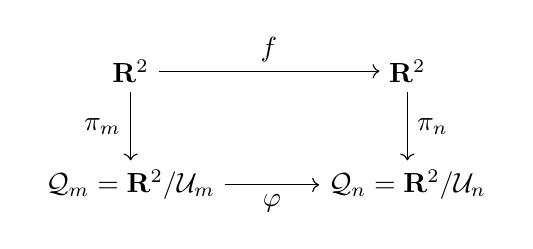
\begin{tikzpicture}[every node/.style={midway}]
    \matrix[column sep={10em,between origins}, row sep={2.5em}] at (0,0) {
    \node(A) {$\RR^2$}  ; & \node (B) {$\RR^2$}; \\
    \node(C) {$\cQ_m = \RR^2/\cU_m$};             & \node (D) {$\cQ_n = \RR^2/\cU_n$};\\
    };
    \draw[->] (A) -- (B) node[auto=left]  {$f$};
    \draw[->] (A) -- (C) node[auto=right]  {$\pi_m$};
    \draw[->] (B) -- (D) node[auto=left] {$\pi_n$};
    \draw[->] (C) -- (D) node[auto=right] {$\varphi$};
  \end{tikzpicture}
\end{center}

This example is the very illustration of the unsuccessful attempt to define smooth maps between orbifolds as locally equivariant maps,
on the level of local symmetry group,
as we mentioned above.

As a side note,
we can understand,
with these two statements,
why it was not obvious at the beginning how to identify smooth maps between orbifolds,
and why the embedding of orbifolds into a category such as \{Diffeology\} could have closed the question.
Of course,
the existence of good smooth maps between orbifolds is crucial for having a covariant satisfactory theory.

\textsc{The Teardrop, An Example of Diffeological Orbifold.} ---
Let us consider the sphere $\S^2 \subset \RR^3 \simeq \CC \times \RR$.
Let $N = (0,1)$ be the North pole.
The following set of parametrizations $\zeta$ defines an orbifold diffeology on $\S^2$ with all points regular,
except the north pole whose structure group is the cyclic group $\cU_m$.
This construction summarized by the Figure \ref{TearDrop},
describes the famous \emph{Teardrop Orbifold},
but as a diffeology.
Let ${U}$ be an Euclidean domain,
$$
  \zeta \colon {U} \to \S^2 \quad \mbox{with} \quad \zeta(r) = \begin{pmatrix}z(r) \\ t(r) \end{pmatrix},
  \quad \mbox{and} \quad |z(r)|^2 + t(r)^2 =1,
  $$
such that, for all $r_0 \in {U}$,

\begin{enumerate}
  \item if $\zeta(r_0) \neq N$,
  then there exists a small ball $\cB$ centered at $r_0$ such that $\zeta \restriction \cB$ is smooth.
  \item If $\zeta(r_0)=N$,
  then there exist a small ball $\cB$ centered at $r_0$ and a smooth parametrization $z$ in $\CC$ defined on $\cB$ such that,
  for all $r\in \cB$,
  $$
    \zeta(r) = {1 \over \sqrt{1 + |z(r)|^{2m}}}\begin{pmatrix} z(r)^m \\ 1 \end{pmatrix}.
    $$
\end{enumerate}

\begin{figure}[th]
  \includegraphics[width=.95\textwidth]{Figures/TearDrop.pdf}
  %\caption{Figure \ref{TearDrop} --- The Teardrop as a diffeological orbifold.}
  \caption{The Teardrop as a diffeological orbifold.}
  \label{TearDrop}
\end{figure}

%%%%%%%%%%%%%%%%%%%%%%%%%%%%%%%%%%%%%%%%%%%%%%%%%%%%%%%%%%
%%
%% MARK: Structure Groupoids of an orbifold
%%
%%%%%%%%%%%%%%%%%%%%%%%%%%%%%%%%%%%%%%%%%%%%%%%%%%%%%%%%%%
\section*{Structure Groupoids of an orbifold.}

In this section,
we associate a \emph{structure groupoid} with each atlas of an orbifold.
Then we show that different atlases give equivalent groupoids:
as categories,
according to Mac Lane definiton \cite{SML78},
and in the sense of Muhly-Renault-Williams \cite{MRW87}.
We give a precise description of the structure groupoid in terms or the groupoid associated with the action of the structure groups $\Gamma$,
and the connecting points of the charts.
This construction is the foundation for a $\CC^*$-algebra associated with the orbifold.
We explicit then a few examples.

\begin{article}\artlabel[Strict Generating Family.] --- Let ${X}$ be an $n$-orbifold and $\cA$ be an atlas.
  Let $f \colon {U} \to {X}$ be a chart,
  then ${U}$ is an open subset of some $\RR^n/\Gamma$ for the D-Topology \cite[\textsection\ 2.8]{PIZ13}.
  Thus $\tilde{U} = \pi^{-1}({U})$ is a $\Gamma$-invariant open subset in $\RR^n$,
  where $\pi \colon \RR^n \to \RR^n/\Gamma$ is the projection.
  Hence,
  ${F} = f \circ \pi$ is a plot of ${X}$.
  We shall call it the \emph{strict lifting} of $f$%
  \footnote{This is compatible with the vocabulary in \cite[\textsection\ 1.54]{PIZ13}.}.
  
  Let $\cF$ be the set of strict liftings ${F} = f \circ \pi$,
  where $f \colon {U} \to {X}$ runs over the charts in $\cA$.
  Then,
  $\cF$ is a generating family of ${X}$.
  We shall say that $\cF$ is the \emph{strict generating family} associated with $\cA$.
\end{article}

\begin{article}\artlabel[Diffeology On The Local Smooth Maps.] --- Let ${X}$ and ${X}'$ be  two diffeological spaces.
  Let $\Cinfty_\loc({X},{X}')$ be the set of local smooth maps from ${X}$ to ${X}'$ \cite[\textsection\ 2.1]{PIZ13}.
  We recall that a map $f$ defined on a subset ${A} \subset {X}$ to ${X}'$ is \emph{local smooth} if ${A}$ is D-open,
  and if $f \colon {A} \to {X}'$ is smooth with ${A}$ equipped with the subset diffeology%
  \footnote{Actually $f$ is local smooth if for every plot $\P$ in ${X}$,
  $f\circ \P$ is a plot of ${X}'$.
  That is the original definition,
  equivalent to the criterion above.}.
  
  Let $\fF$ be the domain of the evaluation of local smooth maps from ${X}$ to ${X}'$,
  $$
    \fF = \{ (f,x) \mid f \in \Cinfty_\loc({X},{X}') \mbox{ and } x \in \dom(f) \}.
    $$
  The evaluation map is,
  as usual,
  $$
    \ev \colon \fF \to {X}' \quad \mbox{with} \quad \ev(f,x) = f(x).
    $$
  
  \textsc{Proposition 1.} ---
  \textit{There exists a coarsest diffeology on $\Cinfty_\loc({X},{X}')$ such that $\ev$ is local smooth.
  That is,
  $\fF$ is D-open in $\Cinfty_\loc({X},{X}') \times {X}$,
  and the map $\ev$ is smooth with $\fF$ equipped with the subset diffeology.
  This diffeology will be called the (standard) \emph{functional diffeology}%
  \footnote{Note that we met already a functional diffeology on local smooth maps,
  that is,
  the functional diffeology on a diffeology \cite[\textsection\ 1.63]{PIZ13}.}.}
  
  Precisely,
  a parametrization $r \mapsto f_r$,
  defined on some Euclidean domain ${U}$,
  is a plot of the functional diffeology if the pre-evaluation map ${F} \colon (r,x) \mapsto f_r(x)$
  defined on
  $$
    \cU = \{ (r,x) \in {U} \times {X} \mid x \in \dom(f_r) \}
    $$
  is local smooth.
  That is,
  if $\cU$ is D-open in ${U} \times {X}$ and ${F} \colon \cU \to {X}'$ is smooth,
  with $\cU$ equipped with the subset diffeology.
  
  Note that the subspace $\Cinfty({X},{X}') \subset \Cinfty_\loc({X},{X}')$ inherits,
  this way,
  the usual functional diffeology \emph{op. cit.} (\textsection 1.57).
  
  \textsc{Proposition 2.} ---
  \textit{The composition of local smooth maps is smooth for the functional diffeology.}
  
  \textsc{Note.} --- This diffeology extends to a \emph{pseudogroup functional diffeology},
  on the pseudogroup of local diffeomorphisms $\Diff_\loc({X})$.
  The parametrization $r \mapsto f_r$ is a plot for this diffeology if it is a plot for the functional diffeology,
  and the inverse plot $r \mapsto f_r^{-1}$,
  where $f_r^{-1}$ is defined from $f_r(\dom(f_r))$ to ${X}$,
  is also a plot for the functional diffeology.
  That insures the smoothness of the inversion $f \mapsto f^{-1}$ in the pseudogroup.
\end{article}

\begin{proof}
  Let us begin to prove that the parametrizations defined above form a diffeology.
  Consider any constant parametrization $r \mapsto f$ where $f \in \Cinfty_\loc({X},{X}')$.
  Thus $\cU = {U} \times \dom(f)$.
  Since $\dom(f)$ is D-open,
  $\cU$ is open in ${U} \times {X}$ and $\ev \colon (r,x)\mapsto f(x)$ is obviously smooth.
  Now,
  let $r \mapsto f_r$ be a plot in $\Cinfty_\loc({X},{X}')$ defined on ${U}$,
  and $s \mapsto r_s$ a smooth parametrization in ${U}$, defined on ${U}'$.
  Consider the smooth map ${F} \colon (s,x) \mapsto (r_s,x)$,
  defined on ${U}' \times {X}$ into ${U} \times {X}$.
  Then,
  $$
    \cU' = \{(s,x) \mid x \in \dom(f_{r_s}) \}
    =  {F}^{-1}\big(\{(r,x) \mid x \in \dom(f_r) \}\big)
    = {F}^{-1}(\cU).
    $$
  Thus,
  $\cU'$ is D-open.
  And again,
  $(s,x) \mapsto f_{r_s}(x)$ is smooth as composition of local smooth maps.
  Finally,
  let $r \mapsto f_r$ a parametrization in $\Cinfty_\loc({X},{X}')$,
  defined on ${U}$,
  that satisfies locally,
  at each point,
  the condition above.
  Let $r \in {U}$,
  there is an open neighborhood $V$ of $r$ such that
  $$
    \cU_{r} = \{ (r',x) \in V \times {X} \mid x \in \dom(f_{r'}) \}
    $$
  is D-open and $\ev \restriction \cU_r$ is local smooth.
  Therefore,
  $\cU = \bigcup_{r\in {U}} \cU_{r}$ is D-open and $\ev \colon \cU \to {X}'$ is local smooth.
  And we have indeed defined a diffeology on $\Cinfty_\loc({X},{X}')$ such that the evaluation map is local smooth.
  
  Now,
  let us prove that this diffeology is the coarsest diffeology such that $\ev \colon \Cinfty_\loc({X},{X}') \times {X} \supset \fF \to  {X}'$ is local smooth.
  Equip $\Cinfty_\loc({X},{X}')$ with any diffeology such that $\ev$ is local smooth%
  \footnote{Note that the set of these diffeologies on $\Cinfty_\loc({X},{X}')$ is not empty since it contains the discrete diffeology.}.
  Let $r \mapsto f_r$ be a plot of $\Cinfty_\loc({X},{X}')$ defined on ${U}$.
  Then,
  the map ${F} \colon (r,x) \mapsto (f_r,x)$,
  from ${U} \times {X}$ to $\Cinfty_\loc({X},{X}') \times {X}$ is smooth.
  Thus,
  the preimage $\cU = {F}^{-1}(\dom(\ev)) = \{(r,x) \mid x \in \dom(f_r)\}$ is D-open in ${U} \times {X}$.
  This is a necessary condition.
  Next,
  let $s \mapsto (r_s,x_s)$ be a plot in $\cU$.
  Since $s \mapsto f_{r_s}$ and $s \mapsto x_s$ are smooth and $x_s \in \dom(f_{r_s})$,
  the composite $s \mapsto f_{r_s}(x_s)$ is smooth.
  Thus,
  the map $(r,x) \mapsto f_r(x)$ defined on $\cU \subset {U} \times {X}$ is local smooth.
  Therefore,
  the diffeology defined above is the coarsest such that the evaluation map is local smooth.
  
  Let us prove finally that the composition is smooth.
  Let ${X},{X}',{X}''$ be three diffeological spaces.
  Let $r\mapsto f_r$ be a plot of $\Cinfty_\loc({X},{X}')$ and $r\mapsto f'_r$ be a plot of $\Cinfty_\loc({X}',{X}'')$,
  both defined on ${U}$.
  With obvious notations,
  let $f \colon {U} \times {X} \supset \cU \to {U} \times {X}'$ and $f' \colon {U} \times {X}' \supset \cU' \to {U} \times {X}''$,
  with $f(r,x)=(r,f_r(x))$ and $f'(r,x')=(r,f'_r(x'))$.
  By hypothesis these two maps are local smooth.
  Thus, their composite $f'' = f' \circ f \colon {U} \times {X} \supset \cU'' \to {U} \times {X}''$ is local smooth \cite[2.2]{PIZ13}.
  But $f''\colon (r,x) \mapsto (r,f_r(x)) \mapsto (r,f'_r(f_r(x)))=(r,f'_r\circ f_r(x))$.
  Thus,
  $r \mapsto f'_r \circ f_r$ is a plot of $\Cinfty_\loc({X},{X}'')$.
  Therefore,
  the composition of local smooth maps is smooth for the functional diffeology.
\end{proof}

\begin{article}\artlabel[The Groupoid Of Germs Of Diffeomorphisms.] ---
  \label{The-Groupoid-Of-Germs-Of-Diffeomorphisms}
  Let ${X}$ be a diffeological space.
  We consider the groupoid of germs of local diffeomorphisms as defined in \cite[\textsection 2.7]{PIZ13}.
  Let us denote it by $\GG$,
  that is,
  $$
    \left\{
    \begin{array}{rcl}
    \Obj(\GG) & = & {X}, \\
    \Mor(\GG) & = & \{\ \germ(\varphi)_x \mid \varphi \in \Diff_\loc({X}) \mbox{ and } x \in \dom(\varphi) \}.
    \end{array}
    \right.
    $$
  The source and target maps are obviously
  $$
    \src(\germ(\varphi)_x) = x \quad \mbox{and} \quad \trg(\germ(\varphi)_x) = \varphi(x).
    $$
  The injection of $\Obj(\GG)$ into $\Mor(\GG)$ is naturally
  $$
    i_{X} \colon x \mapsto \germ(\id_{X})_x.
    $$
  The product of the two germs $\gg=\germ(\varphi)_x$ and $\gg'=\germ(\varphi')_{x'}$,
  with $x'=\varphi(x)$,
  is denoted contravariantly:
  $$
    {\gg}\cdot{\gg'} = \germ(\varphi' \circ \varphi)_x.
    $$
  We consider now the set
  $$
    \fG = \{ (\varphi,x) \mid \varphi \in \Diff_\loc({X}) \mbox{ and } x \in \dom(\varphi) \},
    $$
  equipped with the subset diffeology of the product $\Diff_\loc({X}) \times {X}$,
  where $\Diff_\loc({X})$ is equipped with the functional diffeology defined above.
  We equip then $\Mor(\GG)$ with the pushforward diffeology of $\fG$ by the map
  $$
    \germ \colon (\varphi,x) \mapsto \germ(\varphi)_x.
    $$
  We still call this diffeology, the \emph{functional diffeology}.
  
  \textsc{Proposition.} ---
  \textit{Equipped with the functional diffeology,
  the groupoid $\GG$ is a diffeological groupoid as defined in \cite[\textsection 8.3]{PIZ13}.}
\end{article}

\begin{proof}
  The smoothness of the multiplication and the inversion in $\GG$,
  are directly inherited from the smoothness of the composition and the inversion in the pseudogroup $\Diff_\loc({X})$.
  
  It remains to check that the inclusion $i_{X} \colon x \mapsto \germ(\id_{X})_x$ is smooth.
  Let $\P \colon r \mapsto x_r$ be a plot in ${X}$,
  then $i_{X} \circ \P \colon r \mapsto \germ(\id_{X})_{x_r}$ is the projection of the parametrization $r \mapsto (\id_X,x_r)$ which is obviously a plot of $\fG$.
\end{proof}

\begin{article}\artlabel[The Structure Groupoid Of An Orbifold.] ---
  \label{The-Structure-Groupoid-Of-An-Orbifold}
  Let ${X}$ be an orbifold,
  $\cA$ be an atlas and $\cF$ be the strict generating family over $\cA$.
  Let $\cN$ be the nebula%
  \footnote{See definition in \cite[\textsection\ 1.76]{PIZ13}.}
  of $\cF$,
  that is,
  the sum of the domains of its elements:
  $$
    \cN = \coprod_{{F} \in \cF} \dom({F}).
    $$
  The points $\nu \in \cN$ are the pairs $({F},r)$ such that ${F} \in \cF$ and $r \in \dom({F})$.
  We denote by $\ev$ the natural subduction
  $$
    \ev \colon \cN \to {X} \quad \mbox{with} \quad \ev({F},r) = {F}(r).
    $$
  We consider now the subgroupoid $\GG$ of germs of local diffeomorphisms of $\cN$,
  with the same set of objects $\cN$,
  but whose arrows project along $\ev$,
  on the identity of ${X}$.
  That is,
  $$
    \Mor(\GG) = \{\ \germ(\Phi)_\nu \mid \Phi \in \Diff_\loc(\cN) \mbox{ and } \ev \circ \Phi = \ev \restriction \dom(\Phi) \}.
    $$
  $\Mor(\GG)$ is naturally equipped with the functional diffeology inherited by the full groupoid of germs of local diffeomorphisms.
  Note that,
  given $\Phi \in \Diff_\loc(\cN)$ and $\nu \in \dom(\Phi)$,
  there exists always two plots ${F}$ and ${F}'$ in $\cF$ such that $\nu=({F},r)$ with $r \in \dom({F})$,
  and a local diffeomorphism $\phi$ of $\RR^n$,
  defined on an open ball centered in $r$,
  such that $\dom(\phi) \subset \dom({F})$,
  $\phi = \Phi \restriction \{{F}\}\times \dom({F})$
  and ${F}' \circ \phi = {F} \restriction \dom(\phi)$.
  That is summarized by the diagram:
  $$
    \begin{tikzcd}[column sep=small,every label/.append style = {font = \small}]
    \dom({F}) \supset \dom(\phi) \arrow[dr, swap, "{F}"]  \arrow[rr, "\normalsize \phi"] &    & \dom({F}')\arrow[dl,"{F}'"] \\
    & {X}  &
    \end{tikzcd}
    $$
  We call this groupoid the \emph{Structure Groupoid} of the orbifold ${X}$,
  associated with the atlas $\cA$.
  We shall see below that two different atlases give two equivalent groupoids.
  
  \textsc{Note.} ---
  Consider the groupoid of germs of \emph{local automorphisms} of the evaluation map $\ev \colon \cN \to {X}$.
  That is,
  the germs of all local diffeomorphisms of the nebula that project onto a local diffeomorphism of ${X}$.
  We get then a morphism from this groupoid of automorphisms,
  associated with the atlas $\cA$,
  to the groupoid of local diffeomorphisms of the orbifold ${X}$.
  The structure groupoid $\GG$ defined above is the kernel of this morphism,
  and capture the specificity of the atlas under consideration with respect to another atlas.
\end{article}

\begin{article}\artlabel[Equivalence Of Structure Groupoids]
  \label{Equivalence-Of-Structure-Groupoids}
  Let us recall that a functor $\S \colon {A} \to C$ is an equivalence of categories if and only if,
  $\S$ is full and faithful,
  and each object $c$ in $C$ is isomorphic to $\S(a)$ for some object $a$ in ${A}$ \cite[Chap. 4 \textsection\ 4 Thm. 1]{SML78}.
  For two groupoids $G$ and $G'$ the last condition means that,
  for each object $g'$ in $G'$ there exists an object $g$ in $G$ and an arrow from $g'$ to $\S(g)$ .
  
  Now,
  consider an $n$-orbifold ${X}$.
  Let $\cA$ be an atlas,
  $\cF$ be the associated strict generating family,
  $\cN$ be the nebula of $\cF$ and $\GG$ be the associated structure groupoid.
  Let us describe first the \emph{morphology} of the groupoid.
  To avoid collision between same vocabulary but different meanings in diffeology and groupoid theory,
  we shall call \emph{transitivity-components} of $\GG$ the maximal full subgroupoids of $\GG$ such that each object is connected to any other object by an arrow.
  
  \textsc{Proposition.} ---
  \textit{The fibers of the subduction $\ev \colon \Obj(\GG) \to {X}$ are exactly the transitivity-components of\/ $\GG$.}
  
  \textsc{Theorem.} ---
  \textit{Different atlases of\/ ${X}$ give equivalent groupoids.}
  
  In other words,
  the equivalence class of the structure groupoids of an orbifold is a diffeological invariant.
\end{article}

\begin{proof}
  Let us detail the first proposition.
  First let us recall that $\Obj(\GG)= \cN = \{ ({F},r) \mid {F} \in \cF \mbox{ and } r \in \dom({F}) \}$,
  and $\ev({F},r) = {F}(r)$.
  Next,
  let $x = \ev({F},r) = {F}(r)$ and $x' = \ev({F}',r') = {F}'(r')$.
  Then,
  the proposition states that if $x=x'$,
  then there exists a local diffeomorphism $\varphi$ of $\RR^n$ defined on an open neighborood of $r$ such that,
  $\varphi(r) = r'$ and ${F}' \circ \varphi = {F} \restriction \dom(\varphi)$;
  and the arrow from $({F},r)$ to $({F}',r')$ is $\germ(\varphi)_r$.
  Else,
  if $x \neq x'$ there is no arrow in $\Mor(\GG)$ between $({F},r)$ and $({F}',r')$.
  
  The second part is just obvious,
  by definition of the groupoid $\GG$,
  and the first part is a direct consequence of the Lemma 21 of the article ``Orbifolds As Diffeologies" \cite{IKZ10}.
  Indeed,
  let ${U} = \dom({F})$ and ${U}' = \dom({F}')$.
  Let $V= {U}/\Gamma$ and $f \colon V \to {X}$ be the chart in $\cA$ associated with ${F} \in \cF$.
  Let $V'= {U}'/\Gamma'$ and $f' \colon V' \to {X}$ be the chart in $\cA$ associated with ${F}' \in \cF$.
  There exists a small connected open neighborood $\cO$ of $x$ such that $W = f^{-1}(\cO) \subset V$ and $W' = f'^{-1}(\cO) \subset V'$.
  $$
    \begin{tikzcd}[column sep=1.5em, row sep=3em, every label/.append style = {font = \small}]
    (\tilde{U},r) \arrow{rr}{\tilde\psi}  \arrow[d, swap, "\pi"]       &                         & (\tilde{U}',r') \arrow[d,"\pi'"]           \\
    (W,\pi(r)) \arrow{rr}{\psi} \arrow[dr,swap,"f\restriction W"] &                         & (W',\pi'(r')) \arrow{dl}{f'\restriction W'} \\
    &          (\cO,x)              &
    \end{tikzcd}
    $$
  
  Then,
  $\psi = f'^{-1} \circ f \colon W \to W'$ is a local diffeomorphism from $\RR^n/\Gamma$ to $\RR^n/\Gamma'$ that maps $\pi(r)$ to $\pi'(r')$,
  where $\pi$ and $\pi'$ denote the projections from $\RR^n$ to $\RR^n/\Gamma$ and $\RR^n/\Gamma'$.
  Let $\tilde {U} = \pi^{-1}(W)$ and $\tilde {U}' = \pi'^{-1}(W')$.
  That is exactly the case of the  Lemma cited above:
  \emph{Let $\tilde \psi \colon \tilde{U} \to \tilde{U}'$ be a smooth map that lifts $\psi$,
  then each point of $\tilde{U}$ has a neighborhood on which $\tilde \psi$ is a diffeomorphism with an open subset of $\tilde{U}'$.}
  Thus ${F}' \circ \tilde \psi = {F} \restriction \tilde {U}$,
  and $({F},r)$ and $({F}',r')$ are connected by an arrow of $\GG$,
  that is,
  $\germ(\tilde \psi)_r$,
  see the diagram above.
  
  Now,
  the theorem is quite obvious.
  Let $\cA$ and $\cA'$ be two atlases of ${X}$.
  Consider $\cA'' = \cA \coprod \cA'$.
  With an obvious choice of notations: $\Obj(\GG'')=\Obj(\GG) \coprod \Obj(\GG')$.
  And $\GG''$ contains naturally $\GG$ and $\GG'$ as full subgroupoids.
  The question is then:
  how the adjunction of the crossed arrows between $\GG$ and $\GG'$ changes the distribution of transitivity-components?
  But,
  according to the previous proposition,
  that changes nothing since for $\GG$,
  $\GG'$ or $\GG''$ the set of transitivity-components are always exactly the fibers of the respective subductions $\ev$.
  In other words,
  the set of groupoid components is always ${X}$,
  for any atlas of ${X}$.
  Thus $\GG$ and $\GG'$ are equivalent to $\GG''$,
  therefore $\GG$ and $\GG'$ are equivalent.
\end{proof}

\begin{article}\artlabel[General Description Of The Structure Groupoid.] ---
  \label{General-Description-Of-The-Structure-Groupoid}
  Let ${X}$ be an orbifold.
  Let $\cA$ be an atlas,
  $\cF$ the associated strict generating family with symmetries $\Gamma$,
  and $\GG$ be the associated groupoid.
  We know already that the groupoid components in $\Obj(\GG)$ are the fibers of the projection $\ev \colon ({F},r) \mapsto {F}(r)$.
  Then,
  the (algebraic) structure of the groupoid reduces to the algebraic structure of each full subgroupoid $\GG_x$,
  $x \in {X}$,
  that is,
  $$
    \Obj(\GG_x) = \ev^{-1}(x) \quad \mbox{and} \quad \Mor(\GG_x) =  (\ev \circ \src)^{-1}(x).
    $$
  Let $f$ be a chart in $\cA$,
  let ${U} = \dom(f)$ and $\tilde {U} = \pi^{-1}({U}) \subset \RR^n$ be the domain of its strict lifting ${F} = f \circ \pi \restriction \tilde {U}$,
  where $\pi \colon \RR^n \to \RR^n/\Gamma$.
  Without loss of generality we shall assume that the domains of all charts are connected,
  and then the domain of the strict liftings.
  
  The subgroupoid $\GG_x$ is the assemblage of the subgroupoids $\GG_x^{F}$.
  For all ${F} \in \cF$,
  $$
    \left\{\begin{array}{rcl}
    \Obj(G_x^{F}) & = & \{{F}\} \times \dom({F}), \\
    \Mor(\GG_x^{F}) & = & \{\germ(\varphi)_r \in \Mor(\GG_x) \mid r,\varphi(r) \in \dom({F})  \}.
    \end{array} \right.
    $$
  That is,
  $\Mor(\GG_x^{F}) = \src^{-1}(\Obj(G_x^{F})) \cap \trg^{-1}(\Obj(G_x^{F}))$.
  The assemblage is made first by connecting the groupoid $\GG_x^{F}$ to $\GG_x^{{F}'}$ with any arrow $\germ(\varphi)_r$,
  from $({F},r)$ to $({F}',r')$ such that $x={F}(r)={F}(r')$ and $\varphi(r)=r'$.
  And then spreading the arrows by composition.
  We can represent this construction by a groupoid-set-theoretical diagrams:
  $$
    \GG = \coprod_{x\in {X}} \GG_x \quad \text{and} \quad \GG_x = \GG_x^{F_1} \text{ --- } \GG_x^{F_2} \text{ --- } \cdots \text{ --- } \GG_x^{F_{N_x}}
    $$
  where the $F_i$ are the charts having $x$ in their images and $N_x$ is the number of such charts
  (when the atlas $\cA$ is locally finite).
  The link --- between two groupoids: $G_x^{F_i} \text{ --- } G_x^{F_j}$,
  represents the spreading of the arrows by adjunction of one of them.
  Note that this is absolutely not a smooth representation of $\GG$,
  since the projection $\ev \circ \src \colon \Mor(\GG) \to {X}$ is a subduction.
  And,
  the order of assembly has no influence on the result.
  
  We illustrate this assemblage with the example of a teardrop in Figure~\ref{Assembling-groupoid}.
  The black arrows represent the \emph{elementary groupoids} associated with the two charts of the orbifold.
  The red arrow represents the connecting arrow between the two subgroupoids $\GG_x^{F}$ and $\GG_x^{{F}'}$,
  and the green arrows are obtained by saturation of the groupoid $\GG_x$.
  
  \begin{figure}[t]
    \includegraphics[width=.5\textwidth]{Figures/Assembling-groupoid.pdf}
    %\caption{Figure \ref{Assembling-groupoid} --- Assembling the groupoid of the Teardrop.}
    \caption{Assembling the groupoid of the Teardrop.}
    \label{Assembling-groupoid}
  \end{figure}
  
  Thus,
  the elementary groupoids $G_x^{F}$ are fundamental bricks for the construction of the full groupoid $\GG$.
  
  \textsc{Proposition.} ---
  \textit{The arrows of the groupoid $G_x^{F}$ are the germs of the diffeomorphisms $r \mapsto \gamma \cdot r$,
  where $r \in \dom({F})$ and $\gamma \in \Gamma$. The isotropy group of $r \in \dom({F})$ is the stabilizer  $\Stab_\Gamma(r)$ of $r$ in $\Gamma$.}
  
  In other words, the groupoid $G_x^{F}$ is the groupoid of the action of the local symmetries of the orbifold.
  Note that the structure group at $x\in {X}$,
  defined in \cite[\textsection 4]{IKZ10},
  is exactly the isotropy group (type) of $\GG_x$.
\end{article}

\begin{proof}
  Let $\varphi$ defined on an open ball $\cB$ such that ${F}\circ \varphi = {F} \restriction \cB$,
  which is the condition of the proposition.
  Since ${F} = f \circ \pi$,
  where $f$ is a local diffeomorphism,
  $\pi \circ \varphi(r) = \pi(r)$ for all $r \in \cB$.
  Then,
  for all $r$ in the ball,
  there exists a $\gamma \in \Gamma$ such that $\varphi(r) = \gamma \cdot r$.
  For all $\gamma \in \Gamma$, let
  $$
    \varphi_\gamma \colon \cB \to \RR^n \times \RR^n \quad \mbox{with} \quad \varphi_\gamma(r) = (\varphi(r), \gamma \cdot r).
    $$
  Let $\Delta \subset \RR^n \times \RR^n$ be the diagonal and let us consider
  $$
    \Delta_\gamma = \varphi_\gamma^{-1}(\Delta) = \{ r \in \cB \mid \varphi(r) = \gamma \cdot r \}.
    $$
  \textsc{Lemma 1.} --- There exist at least one $\gamma \in \Gamma$ such that the interior $\mathring{\Delta}_\gamma$ is non empty.
  
  Indeed,
  since $\varphi_\gamma$ is smooth (then continuous),
  the preimage $\Delta_\gamma$ by $\varphi_\gamma$ of the diagonal is closed in $\cB$.
  But,
  the union of all the preimages $\varphi_\gamma^{-1}(\Delta)$ ---~when $\gamma$ runs over $\Gamma$~---
  is the ball $\cB$.
  Then,
  $\cB$ is a finite union of closed subsets.
  According to Baire's theorem,
  there is at least one $\gamma$ such that the interior $\mathring{\Delta}_\gamma$ is not empty.
  
  \textsc{Lemma 2.} --- The union $\mathring{\Delta}_\Gamma = \cup_{\gamma \in \Gamma} \mathring{\Delta}_\gamma$ is an open dense subset of $\cB$.
  
  Indeed,
  let $\cB' \subset \cB$ be an open ball.
  Let us denote with a prime the sets defined above but for $\cB'$.
  Then,
  $\Delta'_\gamma = (\varphi_\gamma  \restriction \cB' )^{-1}(\Delta) = \Delta_\gamma \cap \cB'$,
  and then $\mathring{\Delta}'_\gamma = \mathring{\Delta}_\gamma \cap \cB'$.
  Thus,
  $\cB' \cap \mathring{\Delta}_\Gamma  = \cB' \cap (\cup_{\gamma \in \Gamma} \mathring{\Delta}_\gamma) = \cup_{\gamma \in \Gamma} \mathring{\Delta}'_\gamma$,
  which is not empty for the same reason than $\cup_{\gamma \in \Gamma} \mathring{\Delta}_\gamma$ is not empty.
  Therefore,
  $\mathring{\Delta}_\Gamma$ is dense.
  
  Next,
  and in conclusion:
  the tangent linear map $\D(\varphi) \colon \cB \to \GL(n,\RR)$ is smooth,
  then continuous,
  thus $\D(\varphi)^{-1}(\Gamma)$ is closed.
  But,
  $\D(\varphi)^{-1}(\Gamma)$ contains $\mathring{\Delta}_\Gamma$ which is an open dense subset of $\cB$,
  thus $\D(\varphi)^{-1}(\Gamma) = \cB$.
  Then,
  since $\cB$ is connected, $\D(\varphi)(\cB) \subset \Gamma$ is connected.
  But $\Gamma \subset \GL(n,\RR)$ is discrete,
  then $\D(\varphi)(\cB) = \{ \gamma \}$,
  for some $\gamma \in \Gamma$.
\end{proof}

\begin{article}\artlabel[The Structure Groupoid is Étale and Hausdorff.] ---
  \label{The-Structure-Groupoid-is-Etale-and-Hausdorff}
  The structure groupoid $\GG$ associated with the generating family of an atlas $\cA$ of an orbifold ${X}$ is étale.
  Precisely,
  the projection $\src \colon \Mor(\GG) \to \Obj(\GG)$ is an étale smooth map,
  that is,
  a local diffeomorphism at each point \cite[\textsection 2.5]{PIZ13}.
  For all $\gg \in \Mor(\GG)$ there exists an D-open superset $\cO$ of $\gg$ such that $\src \restriction \cO$ is a diffeomorphism onto its image,
  and the preimages of the elements of $\Obj(\GG)$ by the source map $\src$ are finite.
  %
  Moreover,
  the groupoid $\GG$ is locally compact and Hausdorff.
\end{article}

\begin{proof}
  Let $\gg = \germ(\Phi)_\nu \in \Mor(\GG)$,
  with $\nu = \src(\gg) = ({F},r)$ and $\trg(\gg) = ({F}',r')$.
  Thus,
  $\Phi$ is defined by some $\varphi \in \Diff_\loc(\RR^n)$ with $\dom(\varphi) \subset \dom({F})$,
  $r' = \varphi(r) \in \dom({F}')$ and such that ${F}' \circ \varphi = {F} \restriction \cB$.
  We choose $\varphi \colon \cB \to \dom({F}')$ to be defined on a small ball centered at $r$.
  By an abuse of notation we shall denote $\gg = \germ(\varphi)_r$,
  where $\varphi \in \Diff_\loc(\dom({F}),\dom({F}'))$.
  That is,
  $\varphi$ contains now implicitely the data source and target.
  %
  Now,
  let
  $$
    {F} = f \circ \pi \quad \text{and} \quad {F}' = f' \circ \pi',
    $$
  where $f$ and $f'$ belong to $\cA$,
  $\pi \colon \RR^n \to \RR^n/\Gamma$ and $\pi' \colon \RR^n \to \RR^n/\Gamma'$ are the projections.
  Let $\psi$ be the transition map $f'^{-1} \circ f$,
  then $\pi(r) \in \dom(\psi)$ and $\psi(\pi(r)) = \pi'(r')$.
  Then,
  let
  $$
    \cO = \{ \germ(\varphi)_t \mid t \in \cB \}.
    $$
  Clearly,
  $\src \restriction \cO \colon \germ(\varphi)_t \mapsto t$ is smooth and injective,
  as well as its inverse $t \mapsto \germ(\varphi)_t$.
  Let us show now that $\cO$ is D-open.
  That is,
  for each plot $\P \colon s \mapsto \gg_s$ in $\Mor(\GG)$,
  the subset $\P^{-1}(\cO) \subset \dom(\P)$ is open.
  Let $s \in \P^{-1}(\cO)$,
  that is,
  $\gg_s= \germ(\varphi)_{r_s}$,
  where $r_s=\src(\gg_s)$,
  the discrete index ${F}$ is understood.
  
  Then,
  there exists a small ball $\cV$ centered at $s$ and a plot $s' \mapsto (\varphi_{s'},r_{s'})$,
  defined on $\cV$,
  such that $\gg_{s'} = \germ(\varphi_{s'})_{r_{s'}}$ with $\germ(\varphi_{s})_{r_s}=\germ(\varphi)_{r_s}$ and $r_{s'} \in \cB$.
  Since $s' \mapsto \varphi_{s'}$ is smooth,
  the subset
  $$
    \{(s',r) \in \cV \times \cB \mid r \in \dom(\varphi_{s'}) \}
    $$
  is open.
  Since it contains $(s,r_s)$,
  it contains a product $\cV' \times \cB'$,
  where $\cV'$ is a small ball centered at $s$ and $\cB'$ a small ball centered at $r_s$.
  This implies that for all $s' \in \cV'$,
  $\cB' \subset \dom(\varphi_{s'})$.
  In particular $\cB' \subset \dom(\varphi)$.
  $$
    \begin{tikzcd}[column sep=1.5em, row sep=3em, every label/.append style = {font = \small}]
    \dom({F}) \arrow[rr, dotted, "\varphi_s"]  \arrow[d, swap, "\pi"]       &                         & \dom({F}') \arrow[d,"\pi'"]           \\
    \dom(f) \arrow[rr, dotted, "\psi"] \arrow[dr,swap,"f"] &                         & \dom(f') \arrow{dl}{f'} \\
    &          {X}             &
    \end{tikzcd}
    $$
  Then,
  $\xi_s = \varphi_s \circ \varphi^{-1} \colon \varphi(\cB') \to \dom({F}')$ is a local diffeomorphism of $\dom({F}')$.
  But for all $s'$ one has $\pi' \circ \varphi_{s'} = \psi \circ \pi$,
  wherever it is defined.
  This is shown by the above diagram,
  where the dots denote a local map.
  
  Thus,
  $\pi' \circ \xi_{s'} = \pi'$.
  Thanks to (art. \ref{General-Description-Of-The-Structure-Groupoid}),
  for all $s' \in \cV'$ there is a $\gamma' \in \Gamma'$ such that $\xi_{s'} = \gamma'$.
  But since $\cV'$ is connected and $\Gamma'$ is discrete,
  $\gamma'$ is constant on $\cV'$.
  Now $s \in \cV'$,
  thus,
  for $s'=s$,
  $\gamma' = \varphi^{-1} \circ \varphi_s = \varphi^{-1} \circ \varphi = \id$.
  Hence,
  $\varphi_{s'} = \varphi$ on $\cV'$,
  and $\gg_{s'} = \germ(\varphi)_{r_{s'}}$ on $\cV'$,
  that is,
  $\P(\cV') \subset \cO$.
  Then,
  each $s \in \dom(\P)$ such that $\P(s) \in \cO$ is the center of an open ball whose image is contained in $\cO$.
  Therefore,
  $\P^{-1}(\cO)$ is a union of open balls,
  thus $\P^{-1}(\cO)$ is open and $\cO$ is D-open.
  
  Next,
  let us check that $\Mor(\GG)$ is Hausdorff.
  As above,
  let $\gg = \germ(\varphi)_r \in \Mor(\GG)$.
  We can also represent $\gg$ by a triple $({F},r,\germ(\varphi)_r)$,
  with $\varphi \in \Diff_\loc(\dom({F}),\dom({F}'))$.
  Then,
  let $(G,s,\germ(\psi)_s)$ be another element of $\Mor(\GG)$,
  different from the previous one.
  We separate the situation in three cases:
  ${F} \neq G$,
  ${F} = G$ but $r \neq s$,
  and ${F} = G$, $r = s$ but $\germ(\varphi)_r \neq \germ(\psi)_r$.
  In the two first cases,
  since $\src$ is étale,
  it is sufficient to consider two balls centered around $r$ and $s$ to get two D-open subsets of $\Mor(\GG)$ that separate the two different germs.
  The last case,
  where $({F},r,\germ(\varphi)_r)$ and  $({F},r,\germ(\psi)_r)$ with $\germ(\varphi)_r \neq \germ(\psi)_r$,
  divides in two subcases,
  $\codom(\varphi) \neq \codom(\psi)$ and $\codom(\varphi) = \codom(\psi)$.
  In the first case,
  since the codomains are different,
  it is sufficient to consider a small ball around $r$.
  In the second subcase we consider the composite $f = \psi^{-1} \circ \varphi$ and we apply the Proposition of \art{General-Description-Of-The-Structure-Groupoid}.
  Thus,
  locally $f \colon s \mapsto \gamma \cdot s$,
  for some $\gamma \in \Gamma$,
  the structure group of the orbifold for this plot.
  Since we have assumed $\germ(\varphi)_r \neq \germ(\psi)_r$,
  $\gamma \neq \id$.
  Hence, there is a small ball $\cB$ around $r$ such that $\varphi = \psi \circ \gamma$,
  and therefore the two germs are still separated.
  Therefore,
  $\Mor(\GG)$ is Hausdorff.
\end{proof}

\begin{article}\artlabel[MRW Equivalence Of Structure Groupoids.] ---
  \label{MRW-Equivalence-Of-Structure-Groupoids}
  Let us recall the  Muhly-Renault-Williams equivalence of groupoids \cite[2.1]{MRW87}.
  Let $\GG$ and $\GG'$ be two locally compact groupoids,
  we say that a locally compact space $Z$ is a $(\GG,\GG')$-equivalence if
  \begin{enumerate}
    \item[(i)] $Z$ is a left principal $\GG$-space.
    \item[(ii)] $Z$ is a right principal $\GG'$-space.
    \item[(iii)] The $\GG$ and $\GG'$ actions commute.
    \item[(iv)] The action of $\GG$ on $Z$ induces a bijection of $Z/\GG$ onto $\Obj(\GG')$.
    \item[(v)] The action of $\GG'$ on $Z$ induces a bijection of $Z/\GG'$ onto $\Obj(\GG)$.
  \end{enumerate}
  Let $\src \colon Z \to \Obj(\GG)$ and $\trg \colon Z \to \Obj(\GG')$ be the maps defining the composable pairs associated with the actions of $\GG$ and $\GG'$.
  That is,
  a pair $(\gg,z)$ is composable if $\trg(\gg)=\src(z)$,
  the composite is denoted by $\gg \cdot z$.
  And a pair $(\gg',z)$ is composable if $\src(\gg')=\trg(z)$,
  the composite is denoted by $z \cdot \gg'$.
  
  Let us recall also that an action is principal,
  in the sense of Muhly-Renault-Williams,
  if it is free: $\gg \cdot z = z$ only if $\gg$ is a unit,
  and the \emph{action map} $(\gg, z) \mapsto (\gg \cdot z, z)$,
  defined on the composable pairs,
  is proper  \cite[\textsection 2]{MRW87}.
  
  Now,
  using the hypothesis and notations of \art{Equivalence-Of-Structure-Groupoids},
  let us define $Z$ as the space of germs of local diffeomorphisms,
  from the nebula of the family $\cF$ to the nebula of the family $\cF'$,
  that project on the identity by the evaluation map.
  That is,
  $$
    Z = \left\{ \germ(f)_r \ \bigg\vert \
    \begin{array}{l}
    f \in \Diff_\loc(\dom({F}),\dom({F}'), r \in \dom({F}), \\
    {F} \in \cF, {F}' \in \cF' \text{ and } {F}' \circ f = {F} \restriction \dom(f).
    \end{array} \right\}.
    $$
  Let%
  \footnote{For avoiding a too heaving writing,
  we make an abuse of notation,
  we should precisely write $\src(\germ(f)_r) = ({F}, r)$ and $\trg(\germ(f)_r) = ({F}', f(r))$.}
  $$
    \src(\germ(f)_r) = r \quad \text{and}\quad \trg(\germ(f)_r) = f(r).
    $$
  Then,
  the action of $\gg \in \Mor(\GG)$ on $\germ(f)_r$ is defined by composition if $\trg(\gg)=r$,
  that is,
  $\gg \cdot \germ(f)_r = \germ(f \circ \varphi)_s$,
  where $\gg = \germ(\varphi)_s$,
  $\varphi \in \Diff_\loc(\cN)$ and $\varphi(s) = r$.
  Symmetrically,
  the action of $\gg' \in \Mor(\GG')$ on on $\germ(f)_r$ is defined if $\src(\gg')=f(r)$ by $z \cdot \gg' = \germ(\varphi' \circ f)_r$,
  where $\gg' = \germ(\varphi')_{f(r)}$.
  Then,
  we have:
  
  \textsc{Theorem.} ---
  \textit{The actions of\/ $\GG$ and $\GG'$ on $Z$ are principal,
  and $Z$ is a $(\GG,\GG')$-equivalence in the sense of Muhly-Renault-Williams.}
\end{article}

\begin{proof}
  First of all,
  let us precise that $Z$ is a subspace of the morphisms of groupoid $\GG''$ built in \art{Equivalence-Of-Structure-Groupoids} by adjunction of $\GG$ and $\GG'$,
  and is equipped with the subset diffeology.
  All these groupoids are locally compact and Hausdorff \art{The-Structure-Groupoid-is-Etale-and-Hausdorff}.
  
  Let us check that the action of $\GG$ on $Z$ is free.
  In our case $z=\germ(f)_r$ and $\gg = \germ(\varphi)_s$,
  where $\varphi$ and $f$ are local diffeomorphisms.
  If $\gg \cdot z = z$,
  then obviously $\gg = \germ(\id)_r$.
  
  Next,
  let us denote by $\rho$ the action of $\GG$ on $Z$,
  defined on
  $$
    \GG \star Z = \{(\gg,z) \in \Mor(\GG) \times Z \mid \trg(\gg)=\src(z)\} \quad \text{by} \quad \rho(\gg,z) = \gg \cdot z.
    $$
  This action is smooth because the composition of local diffeomorphisms is smooth,
  and passes onto the quotient groupoid in a smooth operation, see \art{The-Groupoid-Of-Germs-Of-Diffeomorphisms}.
  Moreover, this action is invertible,
  its inverse is defined on
  $$
    Z \star Z = \{(z',z) \in Z \times Z \mid \trg(z')=\trg(z)\} \quad \text{by} \quad \rho^{-1}(z',z) = (\gg=z' \cdot z^{-1},z).
    $$
  In detail,
  $\rho^{-1}(\germ(h)_s, \germ(f)_r) = (\germ(f^{-1} \circ h)_s,\germ(f)_r)$,
  with $f(r)=h(s)$.
  Now,
  the inverse is also smooth when $Z \star Z \subset Z \times Z$ is equipped with the subset diffeology.
  In other words,
  $\rho$ is an induction,
  that is,
  a diffeomorphism from $\GG \star Z$ to $Z \star Z$.
  But since $\GG \star Z$ and $Z \star Z$ are defined by closed relations,
  and $\GG$ and $Z$ are Hausdorff,
  $\GG \star Z$ and $Z \star Z$ are closed into their ambient spaces.
  Thus the intersection of a compact subset in $Z \times Z$ with $Z \star Z$ is compact,
  and then its preimage by the induction $\rho$ is compact.
  Therefore,
  $\rho$ is proper.
  
  It remains to check that the action of $\GG$ on $Z$ induces a bijection of $Z/\GG$ onto $\Obj(\GG')$.
  Let us consider the map $\pi \colon Z \to \Obj(\GG')$ defined by $\pi(\germ(f)_r) = f(r)$.
  Then,
  let $\pi(z)=\pi(z')$,
  with $z=\germ(f)_r$ and $z'=\germ(f')_{r'}$,
  that is,
  $f(r)=f'(r')$.
  But since $f$ and $f'$ are local diffeomorphisms,
  $\varphi = f'^{-1} \circ f$ is a local diffeomorphism with $\varphi(r') = r$.
  Let $\gg = \germ(\varphi)_{r'}$,
  then $\gg \in \Mor(\GG)$ and $z'=\gg \cdot z$.
  Hence,
  the map $\pi$ projects onto an injection from $Z/\GG$ to $\Obj(\GG')$.
  Now,
  let $({F}',r') \in \Obj(\GG')$,
  and let $x = {F}'(r') \in {X}$.
  Since $\cF$ is a generating family,
  there exist $({F},r) \in \Obj(\GG)$ such that ${F}(r)=x$.
  Let $\psi$ and $\psi'$ the charts of ${X}$ defined by factorisation:
  ${F} = \psi \circ \class$ and ${F}' = \psi' \circ \class'$,
  where $\class \colon \RR^n \to \RR^n/\Gamma$ and $\class' \colon \RR^n \to \RR^n/\Gamma'$.
  Let $\xi = \class(r)$ and $\xi' = \class'(r')$.
  Since $\psi(\xi) = \psi'(\xi') = x$,
  $\Psi =_\loc \psi'^{-1} \circ \psi$ is a local diffeomorphism from $\RR^n/\Gamma$ to $\RR^n/\Gamma'$ mapping $\xi$ to $\xi'$.
  Hence,
  according to \cite[Lemma 21]{IKZ10} (recalled in the first section of this paper),
  there exists a local diffeomorphism $f$ from $\dom({F})$ to $\dom({F}')$,
  with some properties of equivariance with respect to $\Gamma$ and $\Gamma'$,
  such that $\class' \circ f = \Psi \circ \class$ and $f(r) = r'$.
  Thus,
  $z = \germ(f)_r$ belongs to $Z$ and $\pi(z)=r'$ (precisely the element $({F}',r')$ of the nebula of $\cF'$).
  Therefore,
  the injective map $\pi$ from $Z/\GG$ to $\Obj(\GG')$ is also surjective,
  and identifies the two spaces.
  Obviously, what has been said on the side $\GG$ can be translated to the side $\GG'$,
  the construction is completely symmetric.
  In conclusion $Z$ satisfies the conditions of a $(\GG,\GG')$-equivalence, in the sense of Muhly-Renault-Williams.
\end{proof}

%%%%%%%%%%%%%%%%%%%%%%%%%%%%%%%%%%%%%%%%%%%%%%%%%%%%%%%%%%
%%
%% MARK: Associated $\CC^*$-Algebra.
%%
%%%%%%%%%%%%%%%%%%%%%%%%%%%%%%%%%%%%%%%%%%%%%%%%%%%%%%%%%%
\section*{The $\CC^*$-Algebras Of An Orbifold}

Let us recall the construction of the $\CC^*$-Algebra associated with a locally compact groupoid $\GG$,
equipped with a Haar system \cite[Part II, \textsection 1]{JR80}.
We consider the particular case where the Haar system is given by the \emph{counting measure},
when the number of arrows emerging from an object is finite.
Let $\cC(\GG)$ be the completion of the compactly supported continuous complex functions on $\Mor(\GG)$,
for the uniform norm.
Let $f$ and $g$ in $\cC(\GG)$,
the convolution and the involution are defined by
$$
  f*g(\gamma) = \sum_{\beta \in \GG^x} f(\beta \cdot \gamma)g(\beta^{-1})
  \quad \mbox{and} \quad f^*(\gamma) = f(\gamma^{-1})^*,
  $$
where  $x = \src (\gamma)$,
and $z^*$ is the conjugate of $z \in \CC$.
The vector space $\cC(\GG)$,
equipped with these operations,
is by definition the $\CC^*$-algebra associated with the groupoid $\GG$.

In the following,
a diffeological groupoid is regarded as a topological groupoid,
equipped with its D-topology%
\footnote{Since smooth maps are D-continuous and diffeomorphism are D-homeomorphisms.}
\cite[\textsection 2.8]{PIZ13}.

\begin{article}\artlabel[The $\CC^*$-Algebra Of An Orbifold.] ---
  \label{The-C*-Algebra-Of-an-Orbifold}
  Let ${X}$ be an orbifold,
  $\cA$ be a atlas and $\GG$ be the structure groupoid associated with $\cA$.
  We suppose that $\cA$ is locally finite to ensure the convergence of the convolution defined above.
  The condition of étale map of the source map \art{The-Structure-Groupoid-is-Etale-and-Hausdorff} ensures the continuity of the convolution product of continuous functions on $\Mor(\GG)$.
  Hence,
  we get this way,
  for each atlas $\cA$ of the orbifold ${X}$,
  the $\CC^*$-algebra $\fA = (\cC(\GG),*)$.
  The dependency of the $\CC^*$-algebra with respect to the atlas is given by the following theorem.
  
  \textsc{Theorem.} ---
  \textit{Different atlases give Morita-equivalent $\CC^*$-algebras.
  Diffeomorphic orbifolds have Morita-equivalent $\CC^*$-algebras.}
  
  In other words,
  we have then defined a functor between the category \{Diffeology\} reduced to diffeomorphisms,
  and the category \{$\CC*$-Algebra\} with morphisms: Morita-equivalences.
\end{article}

\begin{proof}
  Since different atlases give equivalent groupoids in the sense of Muhly-Renault-Williams \art{MRW-Equivalence-Of-Structure-Groupoids},
  and thanks to \cite[Thm. 2.8]{MRW87}, different atlases give strongly Morita-equivalent $\CC^*$-algebras.
  And then obviously,
  diffeomorphic orbifolds have associated strongly Morita-equivalent $\CC^*$-algebras.
\end{proof}

\begin{article}\artlabel[The $\CC^*$-Algebra Of The Simplest Orbifold.] ---
  \label{The-C*-Algebra-Of-The-Simplest-Orbifold}
  Let $\Delta_1= \RR/\{\pm 1\}$.
  This space is obviously the simplest non trivial orbifold.
  It is the only half-line which is an orbifold \cite{PIZ07}.
  The structure of the orbifold is represented by the pushforward of the standard diffeology from $\RR$ to $[0,\infty[$,
  by the square map $\text{sqr} \colon t \mapsto t^2$.
  The singleton $\cF =\{ \text{sqr} \}$ is a strict generating family,
  and the structure groupoid $\GG$ is the groupoid of the action of $\Gamma = \{\pm 1\}$,
  that is,
  $$
    \Obj(\GG) = \RR \quad \mbox{and} \quad \Mor(\GG) = \{ (t,\varepsilon,\varepsilon t) \mid \varepsilon = \pm 1 \} \simeq \RR \times \{\pm 1\}.
    $$
  The groupoid-component structure is represented by the Figure \ref{Delta1}.
  
  A continuous function $f$ on $\Mor(\GG)$ to $\CC$ is a pair of functions $f=(a,b)$,
  where $a(t)=f(t,1)$ and $b(t)=f(t,-1)$.
  With this convention,
  applying the definition reminded in the preamble,
  the convolution product is represented by the matrix multiplication in the module $M_2(\CC) \otimes \cC^0(\RR,\CC)$,
  with
  $$
    f = (a,b) \mapsto M \mbox{ with } M(t) = \begin{pmatrix} a(t) & b(-t) \cr b(t) & a(-t) \end{pmatrix}
    \mbox{ and } M^*(t) = [{}^\tau M(t)]^*,
    $$
  where the supscript $\tau$ represents the transposition and the asterisque denotes the complex conjugation element by element.
  
  \begin{figure}[t]
    \includegraphics[width=.5\textwidth]{Figures/Delta1.pdf}
    %\caption{Figure \ref{Delta1} --- The $\Delta_1$ groupoid, with $\varepsilon \colon t \mapsto -t$.}
    \caption{The $\Delta_1$ groupoid, with $\varepsilon \colon t \mapsto -t$.}
    \label{Delta1}
  \end{figure}
  
  We can already notice that the caracteristic polynomial $\P_M(\lambda)$ of $M$ is invariant by the action of $\{\pm 1\}$,
  and is then defined on the orbifold $\Delta_1$ itself:
  $$
    \P_M(\lambda) \colon t \mapsto \det(M(t)- \lambda \id) = \lambda^2 - \lambda \tr(M(t)) + \det(M(t)),
    $$
  with
  $$
    \tr(M(t)) = a(t) + a(-t) \quad \mbox{and} \quad \det(M(t)) = a(t)a(-t) - b(t)b(-t).
    $$
  Hence,
  from a strict diffeological point of view,
  the structural $\CC^*$-algebra is signed.
\end{article}

\begin{article}\artlabel[The $\CC^*$-Algebra Of The Cone Orbifold.] ---
  \label{The-C*-Algebra-Of-The-Cone-Orbifold}
  As another simple example,
  let us consider the simple cone orbifold $\cQ_3 = \CC/\{1,j,j^2\}$,
  where $j=e^{i2\pi/3}$.
  The structure groupoid is the groupoid of the action of the local symmetries group,
  that is,
  $\Obj(\GG) = \CC$ and $\Mor(\GG) = \CC \times \{1,j,j^2\}$.
  A continuous function $f \colon \Mor(\GG) \to \CC$ is a triple $(a,b,c)$,
  where $a(z)=f(z,1)$, $b(z)=f(z,j)$ and $c(z)=f(z,j^2)$.
  For the same reason as in the previous example,
  the structural $\CC^*$-algebra is represented in the $3 \times 3$ matrices with coefficients in $\cC^0(\CC)$.
  To $f=(a,b,c)$ we associate $z \mapsto M(z)$,
  with
  $$
    M(z) =
    \begin{pmatrix}
    a(z) & c(jz) & b(j^2 z) \cr
    b(z) & a(jx) & c(j^2 z) \cr
    c(z) & b(jz) & a(j^2 z)
    \end{pmatrix}.
    $$
  And this association maps the convolution product to the matrix product.
  The structure of the matrix $M(z)$ extends obviously to the general case of the cone orbifold $\cQ_m$ of any order.
  Now,
  one can check that the caracteristic polynomial function $\P(\lambda) \colon z \mapsto \det(M(z) - \lambda \id)$ is again invariant by the group $\{1,j,j^2\}$,
  and can be regarded as a smooth map from $\cQ_3$ to $\CC$.
\end{article}

%************************************************
%***** Bibliographie
%************************************************

\begin{thebibliography}{YKMZ12}
  
  \bibitem[AC80]{AC80}
  Alain Connes, \emph{$\CC^*$-algèbres et géométrie différentielle}.
  C.R. Acad. Sci. Paris Sér. A-B 290 (1980), pp. A599-A604.
  
  \bibitem[AC95]{AC95}
  Alain Connes.
  \newblock {\em Noncommutative Geometry}.
  \newblock Academic Press, New York, 1995.
  
  \bibitem[PDPI83]{PDPI83}
  \newblock{Paul Donato \& Patrick Iglesias.}
  \newblock{\em Exemple de groupes différentiels~: flots irrationnels sur le tore,}
  \newblock{Preprint CPT-83/P.1524. Centre de Physique Théorique, Marseille, July 1983.}
  \newline
  \newblock{\verb!http://math.huji.ac.il/~piz/documents/EDGDFISLT.pdf!}
  
  \bibitem[PDPI85]{PDPI85}
  \newblock{Paul Donato \& Patrick Iglesias.}
  \newblock{\em Exemple de groupes diff{\'e}ologiques~: flots irrationnels sur le tore.}
  \newblock {Compte Rendu de l'Acad{\'e}mie des Sciences, 301(4), Paris, 1985.}
  
  \bibitem[AH84]{AH84}
  André Haefliger, \emph{Groupoides d'holonomie et classifiants},
  Asterisque \textbf{116} (1984), p.70-97.
  
  \bibitem[PIZ07]{PIZ07}
  \newblock{Patrick Iglesias-Zemmour.}
  \newblock{\em Dimension in Diffeology.}
  \newblock{Indagationes Mathematicae 18(4) 2007.}
  
  \bibitem[PIZ13]{PIZ13}
  \newblock{Patrick Iglesias-Zemmour.}
  \newblock{\em Diffeology.}
  \newblock{Mathematical Surveys and Monographs. The American Mathematical Society, vol. 185, USA R.I. 2013.}
  
  \bibitem[IKZ10]{IKZ10}
  Patrick Iglesias, Yael Karshon and Moshe Zadka.
  \newblock{\em Orbifolds as Diffeology.}
  Transactions of the American Mathematical Society, Volume 362, Number 6, Pages 2811--2831. Providence R.I. June 2010.
  
  \bibitem[YKMZ12]{YKMZ12}
  \newblock{Yael Karshon and Masrour Zoghi.}
  \newblock{\em Orbifold groupoids and their underlying diffeology}.
  E-print, University of Toronto 2012.
  
  \bibitem[SML78]{SML78}
  \newblock{Saunders Mac Lane.}
  \newblock{\emph{Categories for the Working Mathematician}.}
  \newblock{Graduate Texts in Mathematics 5.}
  \newblock{Springer 1978.}
  
  \bibitem[IM02]{IM02}
  Ieke Moerdijk, \emph{Orbifolds as Groupoids: an Introduction},
  in: \emph{Orbifolds in mathematics and physics (Madison, WI, 2001)},
  205--222, Contemp.\ Math.\ \textbf{310}, Amer.\ Math.\ Soc.,
  Providence 2002.
  
  
  \bibitem[MRW87]{MRW87}
  \newblock{Paul Muhly and Jean Renault and Dana Williams.}
  \newblock{\em Equivalence And Isomorphism For Groupoid $\CC^*$-Algebras.}
  \newblock{J. Operator Theory 17, no 1 pp. 3--22. 1987}
  
  \bibitem[JR80]{JR80}
  \newblock{Jean Renault.}
  \newblock{\emph{A groupoid approach to C*-Algebras}.}
  \newblock{Lecture notes in Mathematics (793), Springer-Verlag Berlin Heidelberg New-York 1980.}
  
  \bibitem[MR81]{MR81}
  \newblock{Marc A. Rieffel.}
  \newblock{\em C*-Algebras Associated With Irrational Rotations.}
  \newblock{Pacific Journal of Mathematics, Vol. 93, No. 2, 1981.}
  
  \bibitem[IS56]{IS56}
  \newblock{Ishiro Satake.}
  \newblock{\emph{On a Generalization of the Notion of Manifold},
  Proceedings of the National Academy of Sciences \textbf{42} (1956),
  359--363.}
  
  \bibitem[IS57]{IS57}
  \newblock{Ishiro Satake.}
  \newblock{\emph{The Gauss-Bonnet Theorem for V-manifolds}.
  Journal of the Mathematical Society of Japan, Vol. 9, No. 4,  (1957),
  464--492.}
  
  \bibitem[Sou80]{Sou80}
  \newblock{Jean-Marie Souriau.}
  \newblock{\em Groupes diff\'erentiels.}
  \newblock{Lect. Notes in Math., 836, pp. 91--128.}
  \newblock{Springer Verlag, New-York, 1980.}
  
  \bibitem[WT78]{WT78}
  \newblock{William Thurston.}
  \newblock{\emph{The Geometry and Topology of Three-Manifolds} (Chapter 13).}
  \newblock{Princeton University lecture notes, 1978--1981.}
  
\end{thebibliography}

\end{document}
